\chapter{The Cosmic Microwave Backgound}

\section{The Expanding Universe and the \texorpdfstring{$\Lambda$}{LAMBDA-}CDM Model}
\subsection{The Hubble's Law}\label{ss:hubbleslaw}

In 1929, Edwin Hubble examined the relationship between the distances of
some galaxies and their radial velocities, inferred from their \emph{redshifts},
and formulated an empirical law, which states direct proportionality
between these two quantities (\autoref{fig:hubbleslaw}):

\begin{equation}\label{eq:hubble_law}
        \vb{v} = H_0 \vb{d}
\end{equation}

where $H_0$ is the \emph{Hubble constant}.

\begin{figure}
        \centering
        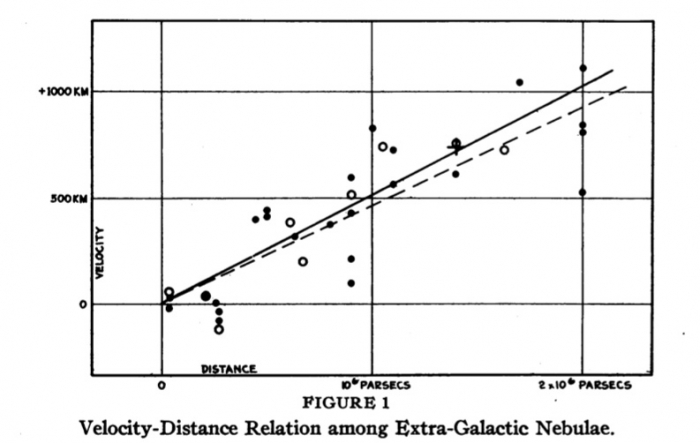
\includegraphics[width=\textwidth]{hubbleslaw}
        \caption{Hubbles Law}
        \label{fig:hubbleslaw}
\end{figure}

The observed \emph{redshifts} couldn't be explained by the proper motion of
the galaxies, instead this phenomenon was caused by the continuos expansion
of our universe.

An expanding universe was first theorized by Friedmann in 1922, before Hubble's
observations, as a consequence of the field equations of the theory of the
\emph{General Relativity} (GR). The starting point of Friedmann derivation was
an elegant and powerful assumption about the structure of our universe:
the \emph{Cosmological Principle}.

\subsection{The Cosmological Principle}\label{ss:cosmological_principle}

The matter in the universe we observe is clustered in gravitationally bound
structures, but observations at large scale (\SI{> 100}{\mega\parsec}) shows
that the place we call home appears to obey the \emph{Cosmological
Principle}:  

\begin{principle}[Cosmological Principle]
        On the largest scales, the universe is spatially homogeneous and isotropic.
\end{principle}

Note that this principle is valid for every possible observer in the
universe. We see an homogeneous and isotropic universe from our planet, and
we believe that any other observer in the universe does: there's no special
place in our universe.

There are two main piece of evidence for the cosmological principle:

\begin{itemize}
        \item The \emph{Comsmic Microwave Background Radiation} (CMB): an almost
        uniform sea of photons which fills all space and provides a snapshot of the
        universe at \num{\sim 380000} years after its birth. The CMB
        presents small fluctuations in temperature with a characteristic
        scale:

        \begin{equation}
                \frac{\var{T}}{T} \sim \num{e-5}
        \end{equation}

        \item A relevant number of \emph{redshift surveys} show that the
        distribution of stars looks increasengly smooth on larger scales.
\end{itemize}

The acceptance of such a profound statement it's the prologue to the
description of the geometry of \emph{spacetime}. 

\subsection{The FLRW Metric}\label{ss:flrw}

Friedmann, Lema\^itre, Robertson and Walker during the 1920-1930s proved
independently that the most generic metric based on the cosmological
principle is the Friedmann-Lema\^itre-Robertson-Walker (FLRW) metric:

\begin{equation}
        \dd{s}^2 = -c^2\dd{t^2} + a\qty(t)^2\qty[\dd{\chi}^2 +
        f_k\qty(\chi)^2\dd{\Omega}^2]
        \label{eq:flrw}
\end{equation}

Where:

\begin{itemize}
        \item $c$ is the speed of light in vacuum;
        \item $a\qty(t)$ is a real function of time known as \emph{scale factor};
        \item $k$ is a real number which parametrizes the spatial curvature of the
        spacetime. Due to the homogeneity and isotropy of space, $k$ is at most a
        function of time. For a fixed time $k$ is a constant and:

        \begin{itemize}
                \item $k = 0$ $\rightarrow$ flat universe;
                \item $k > 0$ $\rightarrow$ open universe;
                \item $k < 0$ $\rightarrow$ closed universe.
        \end{itemize}

        in particular:

        \begin{equation}
                f_k\qty(\chi) =
                        \begin{cases}
                                 \chi & \qif k = 0 \\
                                 \sqrt{k}^{-1} \sin(\sqrt{k} \chi) & \qif k > 0 \\
                                 \sqrt{\abs{k}}^{-1} \sinh(\sqrt{\abs{k}} \chi) & \qif k < 0
                        \end{cases}
        \end{equation}
        \item and $\dd{\Omega}^2 = \dd{\theta}^2 + \sin[2](\theta) \dd{\phi}^2$
        is the metric of the unitary sphere.
\end{itemize}

The FLRW metric in \autoref{eq:flrw} is invariant under the following transformation:

\begin{equation}
        \begin{split}
                \chi & \rightarrow \frac{\chi}{\lambda} \\
                k & \rightarrow \lambda k \\
                a & \rightarrow \lambda a
        \end{split}
\end{equation}

so it is possible to set:

\begin{align}
k & = 0,\pm 1 \\
a\qty(t_0) & = 1
\end{align}

where $t_0$ is the present time and the function $f_k$ becomes: 

        \begin{equation}
                f_k\qty(\chi) =
                        \begin{cases}
                                 \chi & \qif k = 0 \\
                                 \sin \chi & \qif k = 1 \\
                                 \sinh \chi & \qif k = -1 
                        \end{cases}
        \end{equation}

We can immediately note that the valid geometry for an homogeneous
and isotropic spacetime are either flat, spherical or hyperbolic.

\subsection{The Comoving Distance and the Hubble Parameter}

Consider two points in a slice of space in the spacetime ($t = t_*$): $p_1$,
$p_2$. The physical distance between them is calculated using the FLRW
metric for a fixed time:

\begin{equation}
        \dd{s} = a\qty(t_*)\sqrt{\dd{\chi}^2 +
        f_k^2\qty(\chi)\dd{\Omega}^2}
\end{equation}

integrating between $p_1$ and $p_2$, we obtain:

\begin{equation}
        d_{\text{phys}} = a\qty(t_*)d_{\text{co}}
        \label{eq:dd}
\end{equation}

where $d_{\text{co}}$ is the comoving distance, the distance in comoving
coordinates, which expand in the same way as space, and $d_\text{phys}$ is
the proper or physical distance.

Taking the time derivative of \autoref{eq:dd}:

\begin{equation}
        v_{\text{phys}} = \dot a\qty(t) d_{\text{co}} = \frac{\dot a\qty(t)}{a\qty(t)} d_{\text{phys}}
\end{equation}

where $v_{\text{phys}}$ is the physical or proper velocity and the function:

\begin{equation}
        H\qty(t) = \frac{\dot a\qty(t)}{a\qty(t)}
        \label{eq:hubble_parameter}
\end{equation}

is called the \emph{Hubble parameter} and its present day value $H\qty(t_0)
\equiv H_0$ is the \emph{Hubble's constant}, introduced in
\autoref{ss:hubbleslaw}. The Hubble's constant is a cosmological
parameter of our standard cosmological model and has a positive value,
indicating that we live in an expanding universe.

\subsection{The Dynamics of Spacetime}

The evolution of the scale factor $a$ introuced in \autoref{ss:flrw} is
governed by Einstein field equations of GR:

\begin{equation}
        G_{\mu \nu} = \frac{8 \pi G}{c^2} T_{\mu \nu}
        \label{eq:einstein}
\end{equation}

where:

\begin{itemize}
        \item $G_{\mu \nu}$ is the Einstein tensor, which describes the
        geometry of the spacetime;
        \item $G$ is the universal gravitational constant;
        \item $T_{\mu \nu}$ is the energy-momentum tensor, responsible for
        the energy and momentum of matter.
\end{itemize}

Einstein fields equations of GR relate the geometry of the spacetime to the
distribution of matter within it. Assuming the cosmological principle, we
can choose $T_{\mu \nu}$ to be the energy-momentum tensor of a perfect
fluid, which can be completely characterized by its density and pressure:

\begin{equation}
         T_{\mu \nu} = (\rho c^2 + P)u_\mu u_\nu + P g_{\mu \nu} 
         \label{eq:energy_momentum_tensor}
\end{equation}

Substituting \autoref{eq:flrw} and \autoref{eq:energy_momentum_tensor} in
\autoref{eq:einstein}, the field equations reduces to two equations for the
time evolution of the scale factor, known as \emph{Friedmann equations} and
written by Friedmann himself in 1922:

\begin{align}
        \qty(\frac{\dot a\qty(t)}{a\qty(t)})^2 & = \frac{8\pi G}{3} \rho\qty(t)
        - \frac{k\qty(t) c^2}{a^2\qty(t)}
        \label{eq:friedmann_1} \\
        \frac{\ddot a\qty(t)}{a\qty(t)} & = -\frac{4\pi G}{3}
        \qty(\rho\qty(t) + \frac{3 P\qty(t)}{c^2})
        \label{eq:friedmann_2}
\end{align}

The Friedmann equations constitutes a system of two differential equations
with three variables quantity: $a\qty(t)$, $\rho\qty(t)$ and $P\qty(t)$.
The last equation we need to close the system can be deduced from the
conservation of the energy-momentum tensor:

\begin{equation}
        \partial_\mu T^{\mu \nu} = 0 
\end{equation}

It's the \emph{continuity equation}, which express the conservation of energy in a
comsmological setting:

\begin{equation}
        \dot \rho + 3 H \qty(\rho + \frac{P}{c^2}) = 0
        \label{eq:continuity}
\end{equation}

A state equation of the kind $P = P\qty(\rho)$ can be specified to
integrate the continuity equation and determine how the energy density
depends on the scale factor. We guess a generic and simple shape for the
state equation of each component of the cosmological fluid:

\begin{equation}
        P = w \rho c^2 
        \label{eq:state}
\end{equation}

where $w$ is a parameter typical of each component.
Using \autoref{eq:state} in \autoref{eq:continuity} we obtain:

\begin{equation}
        \frac{\dot \rho}{\rho} = -3\qty(1 + w) \frac{\dot a}{a} 
\end{equation}

integrating over time from $t_0$ to a generic time $t$ and using the fact
that $a\qty(t_0) = 1$:

\begin{equation}
        \rho_w\qty(t) = \rho_{w,0} a^{-3\qty(1 + w)} 
\end{equation}

where $\rho_{0,w}$ is the present day energy density.
Therefore the total energy density for the cosmological fluid is:

\begin{equation}
        \rho_{\text{tot}} = \sum_w \rho_w 
\end{equation}

and \autoref{eq:friedmann_1} becomes:

\begin{equation}
        H^2\qty(t) = \frac{8\pi G}{3} \rho_{\text{tot}}\qty(t) -
        \frac{k\qty(t) c^2}{a^2\qty(t)}
\end{equation}

where we have used \autoref{eq:hubble_parameter}. The curvature parameter
$k$ can isolated in the right-hand side of the equation:

\begin{equation}
        \begin{split}
                \frac{k\qty(t) c^2}{a^2\qty(t)} & = 
                \frac{8\pi G \rho_{\text{tot}}\qty(t)}{3} - H^2\qty(t) \\
                \frac{k\qty(t) c^2}{a^2\qty(t)} & = 
                H^2\qty(t) \qty(\frac{8\pi G \rho_{\text{tot}}\qty(t)}{3H^2\qty(t)} - 1) \\
                k(t) & = \frac{H^2\qty(t) a^2\qty(t)}{c^2} \qty(\Omega\qty(t) - 1) \\
        \end{split}
        \label{eq:friedmann_curvature}
\end{equation}

In the last equation we have defined:

\begin{align}
        \rho_c\qty(t) & \equiv \frac{3H^2\qty(t)}{8\pi G} \\
        \Omega\qty(t) & \equiv \frac{\rho_{\text{tot}}\qty(t)}{\rho_c\qty(t)}
\end{align}

The function $\rho_c\qty(t)$ is known as the \emph{critical density}: it
represents the energy density time evolution for a flat universe ($k = 0$).
We note that in this case, the total energy density of the universe is
directly related to the Hubble parameter.

Evaluating \autoref{eq:friedmann_curvature} for $t = t_0$ and assuming a
time independent space curvature $k(t) = k$, yields:

\begin{equation}
        k = \frac{H^2_0}{c^2} \qty(\Omega_0 - 1) \\
\end{equation}

where:

\begin{equation}
        \Omega_0 \equiv \frac{\rho_0}{\rho_{c,0}} = \sum_w
        \frac{\rho_{w,0}}{\rho_{c,0}} \equiv \sum_w \Omega_w
\end{equation}

The adimensional quantities $\Omega_w$ are the \emph{density parameters}
for each fluid component. Note that even though we have omitted the $0$
subscript, the density parameters refer to the fraction of energy observed
today, as the definition implies.

The density parameters sum to:

\begin{equation}
        \sum_w \Omega_w = 1 + \frac{kc^2}{H^2_0} 
\end{equation}

as a consequence, if we live in a flat universe then we must have $\sum_w
\Omega_w = 1$. Any excess energy density, with $\sum_w \Omega_w > 1$ means
that we necessarily live in a positively curved universe with $k = +1$. Any
deficit in energy, with $\sum_w \Omega_w < 1$ gives rise to a negatively
curved $k = 1$ universe. Measuring the present day total energy density 
$\rho_{\text{tot},0}$ and the Hubble constant $H_0$, gives us the
opportunity to have knowledge of the spatial geometry of our universe. 

\subsection{The Components of the Cosmological Fluid}

According to current theories and pieces of evidence, there are three
entities that contribute to the current energy density of our universe:

\begin{itemize}
        \item Conventional matter or \emph{dust};
        \item Radiation;
        \item Dark Energy or \emph{cosmological constant}.
\end{itemize}

To derive a solution for the time evolution of the scale factor $a\qty(t)$
in our universe, it is essential to write a state equation
$P\qty(\rho) = \rho$ for each one of these component:

\begin{itemize}
        \item For dust-like matter (e.g. galaxies or cold dark matter):
        $P_m\qty(\rho_m) = 0$;
        \item For radiation we must impose a null trace for the energy-momentum
        tensor $T_{\mu \nu}$ in \autoref{eq:energy_momentum_tensor}: $P_r\qty(\rho_m)
        = \frac{1}{3} \rho_r c^2$;
        \item For Dark Energy the equation of state is obtained
        substituting  $G_{\mu \nu} = -g_{\mu \nu} \Lambda$, with $\Lambda =
        \text{const.}$ and $\Lambda > 0$, in \autoref{eq:einstein}:
        $P_\Lambda\qty(\rho_\Lambda) = -\rho_\Lambda c^2$, $\rho_\Lambda =
        \frac{\Lambda}{8\pi G}$.
\end{itemize}

The dependence on the scale factor for the energy densities characterized by
these state equations is found making use of the continuity equation 
(\autoref{eq:continuity}):

\begin{align}
        \rho_m\qty(a) & = \rho_{m,0}a^{-3} \label{eq:rho_m} \\
        \rho_r\qty(a) & = \rho_{r,0}a^{-4} \label{eq:rho_r} \\
        \rho_\Lambda\qty(a) & = \rho_{\Lambda,0} \label{eq:rho_lambda} \\
\end{align}

The quantity $\Lambda$ is known as the \emph{cosmological constant} and the
corresponding density $\rho_\Lambda$ is the \emph{vacuum energy density},
associated with the \emph{zero-point energy} of the vacuum state. Note that
Dark Energy has negative pressure $P_\Lambda = -\rho_\Lambda c^2$, and it
does not dilute away as the universe expands.

The total energy density of our universe is:

\begin{equation}
        \rho_\text{tot}\qty(a) = \frac{\rho_{m,0}}{a^3} + \frac{\rho_{r,0}}{a^4} +
        \rho_{\Lambda,0} 
\end{equation}

An expanding universe is radiation dominated at first, in a second phase 
its expansion is driven by matter and at last by Dark Energy. In fact every
universe characterized by a non-zero cosmological constant ($\Lambda \neq
0$) will be ultimately become dodinated by the vacuum energy density
$\rho_\Lambda$. A plot of the evolution of the three kinds of energy
density is shown in \autoref{fig:density_evolution}.

\begin{figure}
        \centering
        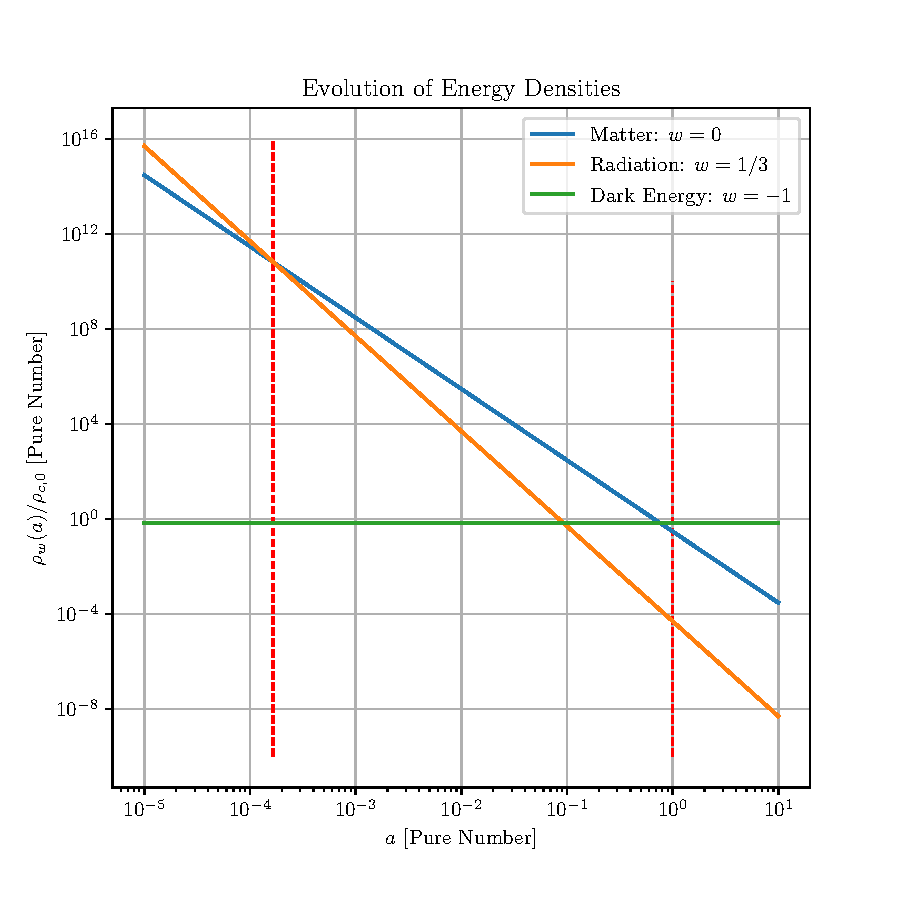
\includegraphics[width=\textwidth]{density_evolution}
        \caption{Energy density evolution.}
        \label{fig:density_evolution}
\end{figure}

Given the total energy density we can solve the first Friedmann equation
and obtain the evolution of the scale factor in our universe. The scale
factors for the three different space curvatures ($k = 0,\pm 1$) in the
simple case of a matter dominated universe are sketched in 
\autoref{fig:scale_factor_evolution_matter}. In the case of an expanding
flat or hyperbolic geometry ($k = 0,-1$) the universe expands for ever with:

\begin{equation}
        \dot a\qty(t \rightarrow +\infty)
                \begin{cases}
                        > 0 & \qif k = -1 \\
                        \rightarrow 0 & \qif k = 0
                \end{cases}
\end{equation}

The spherical universe ($k = +1$) instead eventually re-collapses at a finite
time $t_{\text{bc}}$ with:

\begin{equation}
        a\qty(t_{\text{bc}}) = 0 
\end{equation}

This event is known as \emph{Big Crunch}.

\begin{figure}
        \centering
        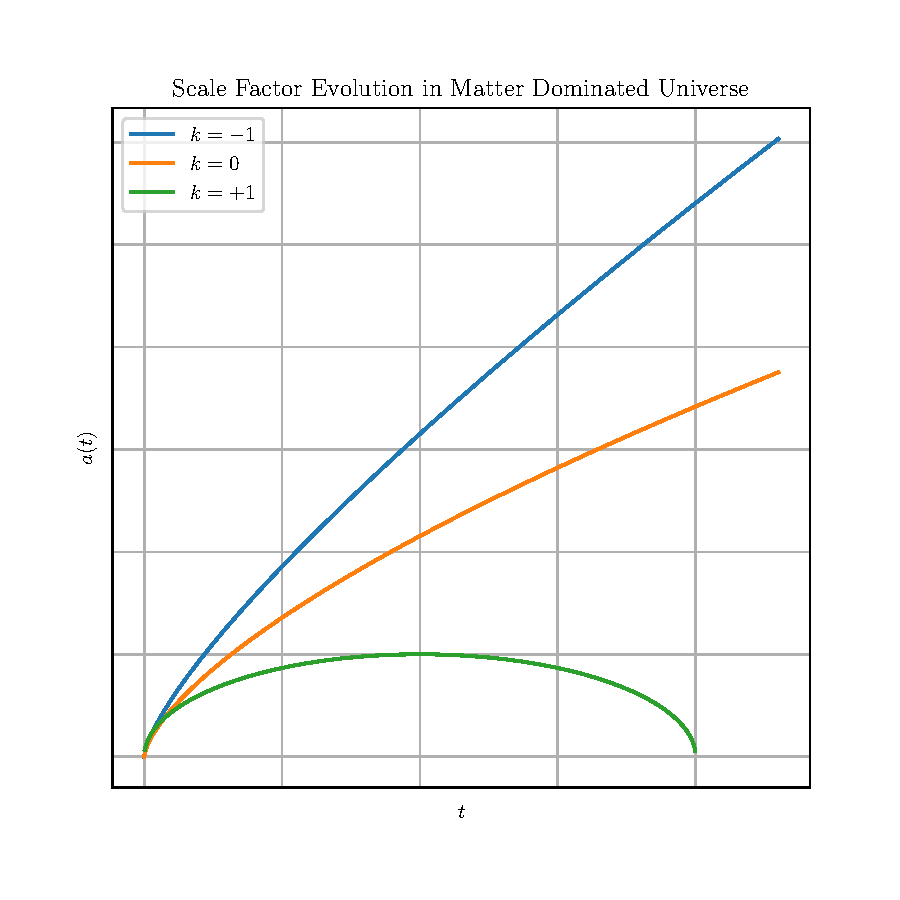
\includegraphics[width=\textwidth]{scale_factor_evolution_matter}
        \caption{Scale factor evolution in a matter dominated universe.}
        \label{fig:scale_factor_evolution_matter}
\end{figure}

In the case of Dark Energy dominated universe every possible solution for
each one of the three space curvatures describes the same spacetime, but with
different coodinates. This spacetime is kwown as \emph{de Sitter space}.
The evolution of the scale factor for this kind of universe is shown in
\autoref{fig:scale_factor_evolution_sitter}. This solution shows a
contracting phase when $t < 0$, followed by a phase of accelerating
expansion ($\ddot a > 0$) when $t > 0$. In particular there's no
\emph{Big Bang} when $t = 0$:

\begin{equation}
        a\qty(t = 0) = \sqrt{\frac{3c^2}{\Lambda}} 
\end{equation}

\begin{figure}
        \centering
        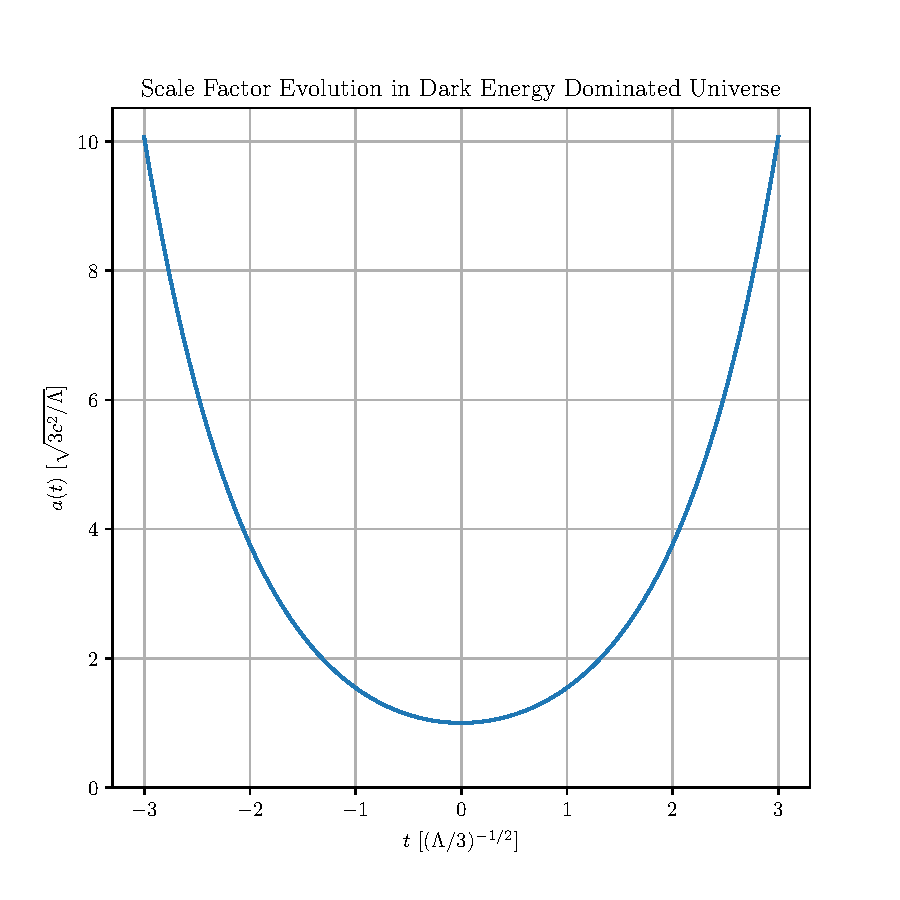
\includegraphics[width=\textwidth]{scale_factor_evolution_sitter}
        \caption{Scale factor evolution for de Sitter space}
        \label{fig:scale_factor_evolution_sitter}
\end{figure}

\subsection{The \texorpdfstring{$\Lambda$}{LAMBDA-}CDM Cosmological Model}

Substituting the expressions for the energy densities of the components of
the cosmological fluid (\autoref{eq:rho_m}, \autoref{eq:rho_r} and
\autoref{eq:rho_lambda}) in \autoref{eq:friedmann_1} yields the second
Friedmann equation for our universe:

\begin{equation}
        H^2\qty(t) = \frac{8\pi G}{3} \qty(\frac{\rho_{m,0}}{a^3\qty(t)} +
        \frac{\rho_{r,0}}{a^4\qty(t)} + \rho_{\Lambda,0}) -
        \frac{k\qty(t) c^2}{a^2\qty(t)}
\end{equation}

If the first term in the right-hand side is multiplied and
divided by the squared hubble constant $H^2_0$, the equation is parametrized
by the density parameters $\Omega_w$:

\begin{equation}
        H^2\qty(t) = H^2_0 \qty(\frac{\Omega_m}{a^3\qty(t)} +
        \frac{\Omega_r}{a^4\qty(t)} + \Omega_\Lambda) -
        \frac{k\qty(t) c^2}{a^2\qty(t)}
\end{equation}

The collection of the numbers $\Omega_m$, $\Omega_r$, $\Omega_\Lambda$ and
$k$ goes by the name of the \emph{$\Lambda$CMD model}, with $\Lambda$
denoting the cosmological constand and CMD denoting \emph{cold dark matter}.
The great interest in the study of the Cosmic Microwave Background resides
in the fact that the values of the parameters of the $\Lambda$CMD
cosmological model can be extracted from observations of this relic
radiation.

\section{The CMB Radiation}

This section is devoted to the introduction of the Comsmic Microwave
Background (CMB) Radiation. To understand what caused the CMB radiation to
emerge, we start describing what we think happened in the universe from the
first instants after the Big Bang to today.

\subsection{A Brief Thermal History of Our Universe}\label{ss:brief_thermal_history}

The essence of the hot Big Bang theory is simply to go back in time taking
the temperature scaling $T \sim \frac{1}{a}$. As the solution for the scale
factor suggests, as we go further back in time, more the temperature and
the energy density of the universe increase and more species join the
primordial plasma reaching the thermodinamic equilibrium. As we know in the
early stages the universe was radiation dominated, so the temperature and
energy density decreased according to:

\begin{equation}
        T\qty(t), \rho\qty(t) \propto t^{-\frac{1}{2}}         
\end{equation}

A summary of some of the key events in the early history of the universe
follows:

\begin{itemize}
        \item \textbf{Electroweak phase transition:} \SI{e-12}{\second},
        \SI{e22}{\kelvin}

        At this time the electroweak phase transition occured, separating
        the weak and electromagnetic interactions. In this epoch the
        universe was filled with a quark-gluon plasma.
        \item \textbf{QCD phase transition:} \SI{e-6}{\second},
        \SI{e16}{\kelvin}

        At this time the average energy of particles interaction had fallen
        below the mass of the adrons. In this epoch the temperature was
        high enough that hadrons and anti-hadrons pairs could form. Later
        new pairs were no longer produced and most of the hadrons and
        anti-hadrons annihilated. Due to the matter and anti-matter
        assimmetry a small portion of hadrons remained in the universe. 

        At this time the universe was filled with neutrons and protons in
        the ratio of:

        \begin{equation}
                \frac{n_n}{n_p} = \frac{1}{5} 
        \end{equation}

        due to the small mass difference between the two particles. Later
        this ratio became smaller as a consequence of the neutron $\beta$
        decay:

        \begin{equation}
                n \rightarrow p + e^- + \bar\nu_e 
        \end{equation}

        and its present day value is:

        \begin{equation}
                \frac{n_n}{n_p} = \frac{1}{7} 
        \end{equation}

        \item \textbf{Neutrino Decoupling:} \SI{1}{\second},
        \SI{e10}{\kelvin}

        At this time neutrinos decoupled from the primordial plasma and
        began to travel freely into space. As neutrinos rarely interact
        with matter, they still exist today as the Cosmic
        Neutrino Background (C$\nu$B), analogous to the much later Cosmic
        Microwave Background emitted during recombination.

        \item \textbf{$e^-e^+$ Annihilation:} \SI{6}{\second},
        \SI{5e9}{\kelvin}

        At this time the average energy of photons became less then the rest mass
        of the electron-positron pairs and the reaction:

        \begin{equation}
                2\gamma \rightleftharpoons e^- + e^+
        \end{equation}

        fell out of equilibrium. The left $e^-e^+$ pairs annihilated and,
        due to the matter and anti-matter asimmetry, just a small portion
        of electrons survived.

        \item \textbf{Nucleosynthesis:} \SI{3}{\minute}, \SI{e9}{\kelvin}

        At this time the tempearture and pressure of the universe allowed
        the stabilization of deuterium and the consequent formation of
        light nuclei, such as hydrogen and its isotopes
        (\SI{\sim 75}{\percent}) and helium (\SI{\sim 25}{\percent}).

        \item \textbf{Matter-Radiation Equality:} \SI{50000}{\year},
        \SI{8700}{\kelvin}

        At this time the universe became matter dominated: the energy
        density of matter $\rho_m$ became equal to the energy density of
        radiation $\rho_r$ (\autoref{fig:density_evolution}).

        \item \textbf{Recombination and Last Scattering:} \SI{370000}{\year},
        \SI{3000}{\kelvin}

        At this time the universe has cooled enough ($k_bT <<
        \SI{13.6}{\electronvolt}$) to allow the formation of the first
        neutral atoms. This event is known as \emph{recombination} and it is
        associated to the photons decoupling or \emph{last scattering}, that
        refers to the mean free path of photons in the universe becoming
        infinite. Nowadays the last scattering photons are still propagating in
        space and we refer to them as the \emph{Cosmic Microwave Background}.

        \item \textbf{Matter-Dark Energy Equality:} \SI{e10}{\year},
        \SI{3.8}{\kelvin}

        At this time the universe became dominated by Dark Matter: the
        vacuum energy density $\rho_\Lambda$ became equal to the energy density of
        matter $\rho_m$ (\autoref{fig:density_evolution}), determining a
        phase of accelerated expansion.

        \item \textbf{Today:} \SI{1.38e10}{\year}, \SI{2.7}{\kelvin}

        The epoch we live in.
\end{itemize}

\begin{figure}
        \centering
        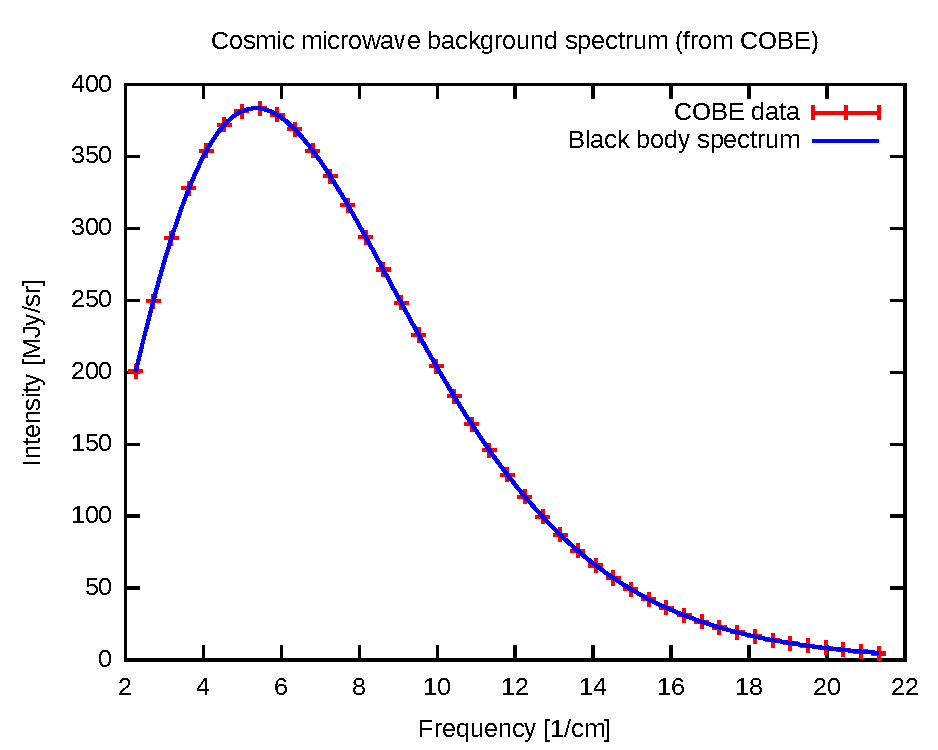
\includegraphics[width=\textwidth]{CMB_Spectrum_COBE}
        \caption{CMB Spectrum COBE}
        \label{fig:cmb_spectrum_cobe}
\end{figure}

\section{The CMB Temperature Anisotropies}

\begin{figure}
        \centering
        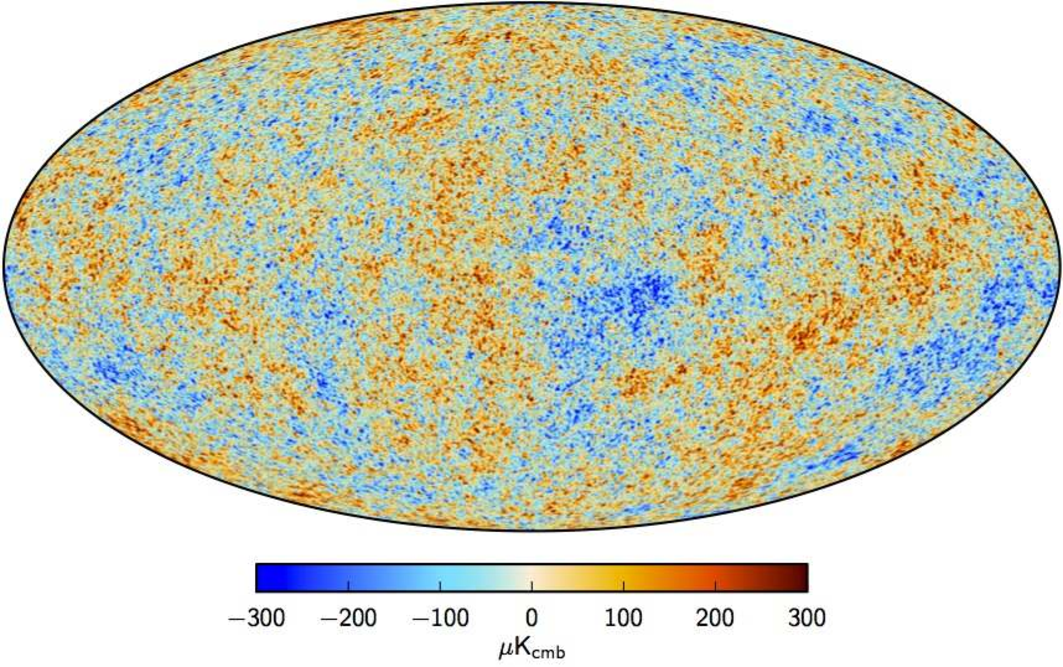
\includegraphics[width=\textwidth]{Planck_CMB}
        \caption{CMB Anisotropies Planck}
        \label{fig:plack_cmb}
\end{figure}

\section{The CMB Polarization}
